\documentclass{standalone}
\usepackage{tikz}
\usetikzlibrary{patterns, positioning}


\begin{document}
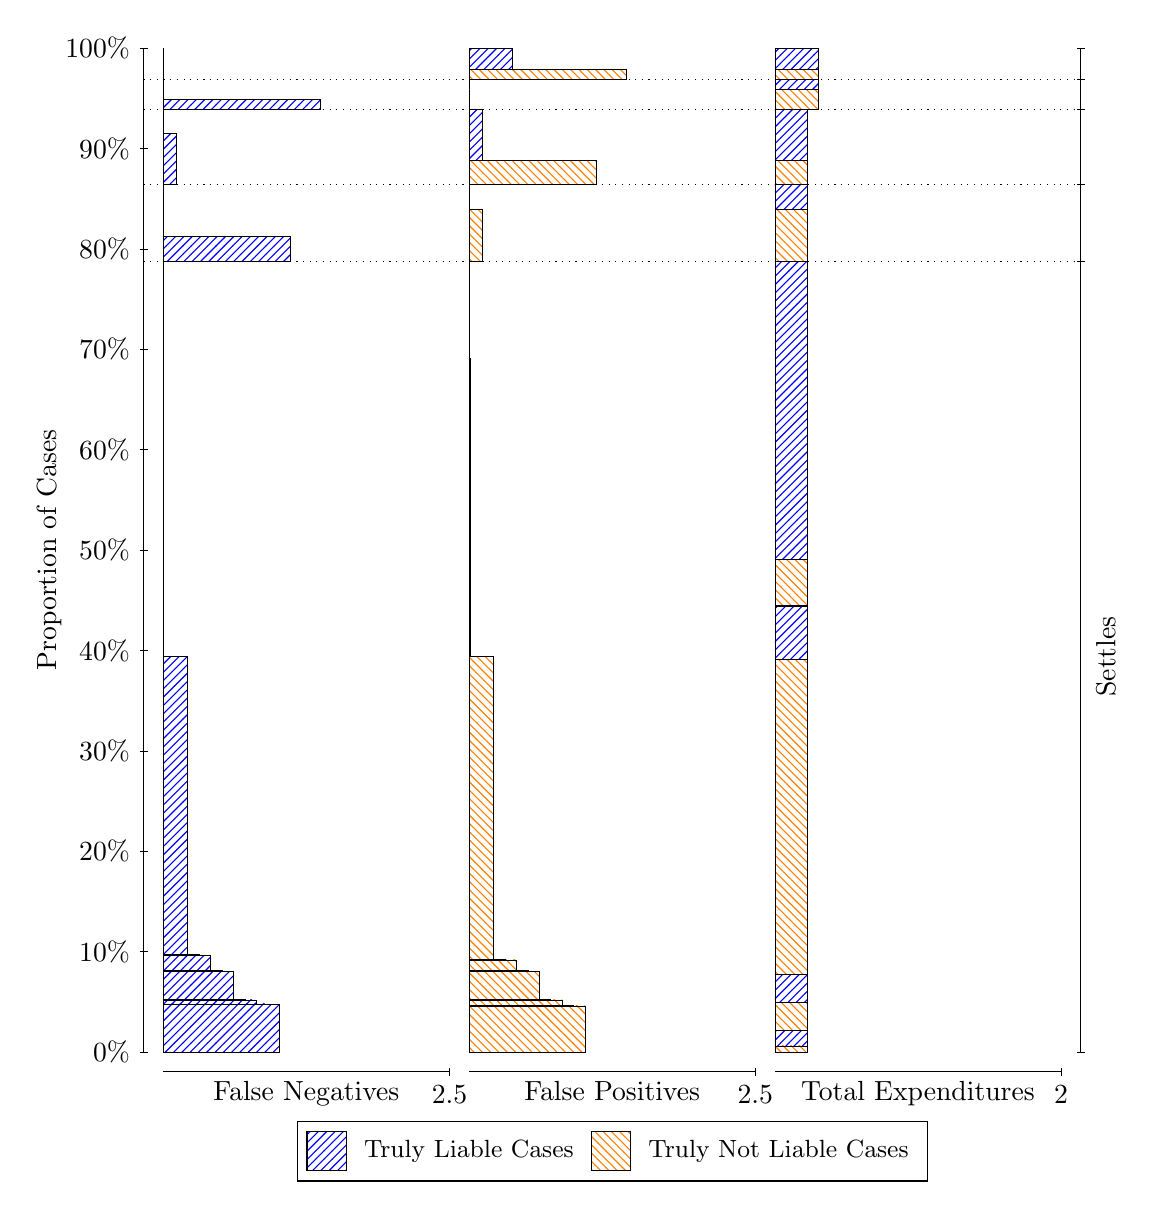
\begin{tikzpicture}
\draw[black, very thin] (1.5,1.75) -- (1.5,14.5);
\node[rotate=90, text=black, anchor=center] at (0.3, 8.125) {Proportion of Cases};
\draw[black, very thin] (1.45,1.75) -- (1.55,1.75);
\node[text=black, anchor=east] at (1.45, 1.75) {0\%};
\draw[black, very thin] (1.45,3.025) -- (1.55,3.025);
\node[text=black, anchor=east] at (1.45, 3.025) {10\%};
\draw[black, very thin] (1.45,4.3) -- (1.55,4.3);
\node[text=black, anchor=east] at (1.45, 4.3) {20\%};
\draw[black, very thin] (1.45,5.575) -- (1.55,5.575);
\node[text=black, anchor=east] at (1.45, 5.575) {30\%};
\draw[black, very thin] (1.45,6.85) -- (1.55,6.85);
\node[text=black, anchor=east] at (1.45, 6.85) {40\%};
\draw[black, very thin] (1.45,8.125) -- (1.55,8.125);
\node[text=black, anchor=east] at (1.45, 8.125) {50\%};
\draw[black, very thin] (1.45,9.4) -- (1.55,9.4);
\node[text=black, anchor=east] at (1.45, 9.4) {60\%};
\draw[black, very thin] (1.45,10.675) -- (1.55,10.675);
\node[text=black, anchor=east] at (1.45, 10.675) {70\%};
\draw[black, very thin] (1.45,11.95) -- (1.55,11.95);
\node[text=black, anchor=east] at (1.45, 11.95) {80\%};
\draw[black, very thin] (1.45,13.225) -- (1.55,13.225);
\node[text=black, anchor=east] at (1.45, 13.225) {90\%};
\draw[black, very thin] (1.45,14.5) -- (1.55,14.5);
\node[text=black, anchor=east] at (1.45, 14.5) {100\%};

\draw[black, very thin] (13.4,1.75) -- (13.4,14.5);
\draw[black, very thin] (13.35,1.75) -- (13.45,1.75);
\node[anchor=west] at (13.35, 1.75) {};
\draw[black, very thin] (13.35,11.794) -- (13.45,11.794);
\node[anchor=west] at (13.35, 11.794) {};
\draw[black, very thin] (13.35,12.77) -- (13.45,12.77);
\node[anchor=west] at (13.35, 12.77) {};
\draw[black, very thin] (13.35,13.719) -- (13.45,13.719);
\node[anchor=west] at (13.35, 13.719) {};
\draw[black, very thin] (13.35,14.105) -- (13.45,14.105);
\node[anchor=west] at (13.35, 14.105) {};
\draw[black, very thin] (13.35,14.5) -- (13.45,14.5);
\node[anchor=west] at (13.35, 14.5) {};

\draw[black, very thin, pattern color=blue, pattern=north east lines] (1.75,1.75) rectangle (3.2215,2.3576);
\draw[black, very thin, pattern color=blue, pattern=north east lines] (1.75,2.3576) rectangle (3.0762,2.3618);
\draw[black, very thin, pattern color=blue, pattern=north east lines] (1.75,2.3618) rectangle (2.9308,2.4127);
\draw[black, very thin, pattern color=blue, pattern=north east lines] (1.75,2.4127) rectangle (2.7855,2.4183);
\draw[black, very thin, pattern color=blue, pattern=north east lines] (1.75,2.4183) rectangle (2.7855,2.4192);
\draw[black, very thin, pattern color=blue, pattern=north east lines] (1.75,2.4192) rectangle (2.6402,2.7748);
\draw[black, very thin, pattern color=blue, pattern=north east lines] (1.75,2.7748) rectangle (2.4948,2.7866);
\draw[black, very thin, pattern color=blue, pattern=north east lines] (1.75,2.7866) rectangle (2.3495,2.9727);
\draw[black, very thin, pattern color=blue, pattern=north east lines] (1.75,2.9727) rectangle (2.2042,2.9863);
\draw[black, very thin, pattern color=blue, pattern=north east lines] (1.75,2.9863) rectangle (2.0588,6.7713);
\draw[black, very thin, pattern color=orange, pattern=north west lines] (1.75,6.7713) rectangle (1.75,11.794);
\draw[black, very thin, pattern color=blue, pattern=north east lines] (1.75,11.794) rectangle (3.3668,12.11);
\draw[black, very thin, pattern color=orange, pattern=north west lines] (1.75,12.11) rectangle (1.75,12.77);
\draw[black, very thin, pattern color=blue, pattern=north east lines] (1.75,12.77) rectangle (1.9135,13.413);
\draw[black, very thin, pattern color=orange, pattern=north west lines] (1.75,13.413) rectangle (1.75,13.719);
\draw[black, very thin, pattern color=blue, pattern=north east lines] (1.75,13.719) rectangle (3.7483,13.848);
\draw[black, very thin, pattern color=orange, pattern=north west lines] (1.75,13.848) rectangle (1.75,14.105);
\draw[black, very thin, pattern color=orange, pattern=north west lines] (1.75,14.105) rectangle (1.75,14.233);
\draw[black, very thin, pattern color=blue, pattern=north east lines] (1.75,14.233) rectangle (1.75,14.5);
\draw[black, very thin, pattern color=orange, pattern=north west lines] (5.6333,1.75) rectangle (7.1048,2.3352);
\draw[black, very thin, pattern color=orange, pattern=north west lines] (5.6333,2.3352) rectangle (6.9595,2.3404);
\draw[black, very thin, pattern color=orange, pattern=north west lines] (5.6333,2.3404) rectangle (6.8142,2.4113);
\draw[black, very thin, pattern color=orange, pattern=north west lines] (5.6333,2.4113) rectangle (6.6688,2.4169);
\draw[black, very thin, pattern color=orange, pattern=north west lines] (5.6333,2.4169) rectangle (6.5235,2.7708);
\draw[black, very thin, pattern color=orange, pattern=north west lines] (5.6333,2.7708) rectangle (6.3782,2.7863);
\draw[black, very thin, pattern color=orange, pattern=north west lines] (5.6333,2.7863) rectangle (6.2328,2.9196);
\draw[black, very thin, pattern color=orange, pattern=north west lines] (5.6333,2.9196) rectangle (6.0875,2.9305);
\draw[black, very thin, pattern color=orange, pattern=north west lines] (5.6333,2.9305) rectangle (5.9422,6.7731);
\draw[black, very thin, pattern color=blue, pattern=north east lines] (5.6333,6.7731) rectangle (5.6515,10.558);
\draw[black, very thin, pattern color=blue, pattern=north east lines] (5.6333,10.558) rectangle (5.6333,11.794);
\draw[black, very thin, pattern color=orange, pattern=north west lines] (5.6333,11.794) rectangle (5.7968,12.455);
\draw[black, very thin, pattern color=blue, pattern=north east lines] (5.6333,12.455) rectangle (5.6333,12.77);
\draw[black, very thin, pattern color=orange, pattern=north west lines] (5.6333,12.77) rectangle (7.2502,13.076);
\draw[black, very thin, pattern color=blue, pattern=north east lines] (5.6333,13.076) rectangle (5.7968,13.719);
\draw[black, very thin, pattern color=orange, pattern=north west lines] (5.6333,13.719) rectangle (5.6333,13.976);
\draw[black, very thin, pattern color=blue, pattern=north east lines] (5.6333,13.976) rectangle (5.6333,14.105);
\draw[black, very thin, pattern color=orange, pattern=north west lines] (5.6333,14.105) rectangle (7.6317,14.233);
\draw[black, very thin, pattern color=blue, pattern=north east lines] (5.6333,14.233) rectangle (6.1783,14.5);
\draw[black, very thin, pattern color=orange, pattern=north west lines] (9.5167,1.75) rectangle (9.9254,1.8261);
\draw[black, very thin, pattern color=blue, pattern=north east lines] (9.5167,1.8261) rectangle (9.9254,2.0258);
\draw[black, very thin, pattern color=orange, pattern=north west lines] (9.5167,2.0258) rectangle (9.9254,2.3796);
\draw[black, very thin, pattern color=blue, pattern=north east lines] (9.5167,2.3796) rectangle (9.9254,2.7352);
\draw[black, very thin, pattern color=orange, pattern=north west lines] (9.5167,2.7352) rectangle (9.9254,6.7367);
\draw[black, very thin, pattern color=blue, pattern=north east lines] (9.5167,6.7367) rectangle (9.9254,7.405);
\draw[black, very thin, pattern color=orange, pattern=north west lines] (9.5167,7.405) rectangle (9.9254,7.4114);
\draw[black, very thin, pattern color=blue, pattern=north east lines] (9.5167,7.4114) rectangle (9.9254,7.4242);
\draw[black, very thin, pattern color=orange, pattern=north west lines] (9.5167,7.4242) rectangle (9.9254,8.0094);
\draw[black, very thin, pattern color=blue, pattern=north east lines] (9.5167,8.0094) rectangle (9.9254,11.794);
\draw[black, very thin, pattern color=orange, pattern=north west lines] (9.5167,11.794) rectangle (9.9254,12.455);
\draw[black, very thin, pattern color=blue, pattern=north east lines] (9.5167,12.455) rectangle (9.9254,12.77);
\draw[black, very thin, pattern color=orange, pattern=north west lines] (9.5167,12.77) rectangle (9.9254,13.076);
\draw[black, very thin, pattern color=blue, pattern=north east lines] (9.5167,13.076) rectangle (9.9254,13.719);
\draw[black, very thin, pattern color=orange, pattern=north west lines] (9.5167,13.719) rectangle (10.062,13.976);
\draw[black, very thin, pattern color=blue, pattern=north east lines] (9.5167,13.976) rectangle (10.062,14.105);
\draw[black, very thin, pattern color=orange, pattern=north west lines] (9.5167,14.105) rectangle (10.062,14.233);
\draw[black, very thin, pattern color=blue, pattern=north east lines] (9.5167,14.233) rectangle (10.062,14.5);
\draw[black, dotted] (1.5,11.794) -- (13.4,11.794);
\draw[black, dotted] (1.5,12.77) -- (13.4,12.77);
\draw[black, dotted] (1.5,13.719) -- (13.4,13.719);
\draw[black, dotted] (1.5,14.105) -- (13.4,14.105);
\draw[black, very thin] (1.75,1.5) -- (5.3833,1.5);
\node[text=black, anchor=north] at (3.5667, 1.5) {False Negatives};
\draw[black, very thin] (5.3833,1.45) -- (5.3833,1.55);
\node[text=black, anchor=north] at (5.3833, 1.45) {2.5};

\draw[black, very thin] (5.6333,1.5) -- (9.2667,1.5);
\node[text=black, anchor=north] at (7.45, 1.5) {False Positives};
\draw[black, very thin] (9.2667,1.45) -- (9.2667,1.55);
\node[text=black, anchor=north] at (9.2667, 1.45) {2.5};

\draw[black, very thin] (9.5167,1.5) -- (13.15,1.5);
\node[text=black, anchor=north] at (11.333, 1.5) {Total Expenditures};
\draw[black, very thin] (13.15,1.45) -- (13.15,1.55);
\node[text=black, anchor=north] at (13.15, 1.45) {2};

\node[text=black, centered, rotate=90] at (13.72, 6.7722) {Settles};





\draw (7.449999999999999,1.5) node[draw=none] (baseCoordinate) {};
\begin{scope}[align=center]
        \matrix[scale=0.5, draw=black, below=0.5cm of baseCoordinate, nodes={draw}, column sep=0.1cm]{
            \node[rectangle, draw, minimum width=0.5cm, minimum height=0.5cm, pattern color=blue, pattern=north east lines] {}; &
            \node[draw=none, font=\small, text=black] (B) {Truly Liable Cases}; &
            \node[rectangle, draw, minimum width=0.5cm, minimum height=0.5cm, pattern color=orange, pattern=north west lines] {}; &
            \node[draw=none, font=\small, text=black] (B) {Truly Not Liable Cases}; \\
            };
\end{scope}

\end{tikzpicture}
\end{document}